\documentclass[10pt, a4paper]{article}


\newcommand{\enname}{Chinatip Lawansuk}
\newcommand{\zhname}{廖有福}
\newcommand{\telnum}{+886987422475}
\newcommand{\email}{l.chinatip@gmail.com}
\newcommand{\linkedin}{https://www.linkedin.com/in/chinatip-lawansuk-2b6718199/}
\newcommand{\git}{https://github.com/chinatip-l}
\newcommand{\gitname}{chinatip-l}
\newcommand{\doi}{10.1109/ICCE59016.2024.10444315}
\newcommand{\doilink}{https://doi.org/\doi}


% Packages:
\usepackage[
    ignoreheadfoot, % set margins without considering header and footer
    top=0.75 cm, % seperation between body and page edge from the top
    bottom=0.75 cm, % seperation between body and page edge from the bottom
    left=0.75 cm, % seperation between body and page edge from the left
    right=0.75 cm, % seperation between body and page edge from the right
    footskip=0 cm, % seperation between body and footer
    % showframe % for debugging 
]{geometry} % for adjusting page geometry

\usepackage{graphicx}
\usepackage{xeCJK}
\usepackage{pdfpages}

% \setmainfont{fonts/static/NotoSerif-Regular.ttf}
\setmainfont{NotoSerif}[
    UprightFont    = NotoSerif-Regular.ttf,
    BoldFont       = NotoSerif-Bold.ttf,
    ItalicFont     = NotoSerif-Italic.ttf,
    BoldItalicFont = NotoSerif-BoldItalic.ttf,
    Path           = fonts/static/
]
\setCJKmainfont{NotoSerifTC}[
    UprightFont    = NotoSerifTC-Regular.ttf,
    BoldFont       = NotoSerifTC-ExtraBold.ttf,
    Path           = fonts/static/
]




\usepackage{titlesec} % for customizing section titles
\usepackage{tabularx} % for making tables with fixed width columns
\usepackage{array} % tabularx requires this
\usepackage[dvipsnames]{xcolor} % for coloring text
\definecolor{primaryColor}{RGB}{0, 0, 0} % define primary color
\usepackage{enumitem} % for customizing lists
\usepackage{fontawesome5} % for using icons
\usepackage{amsmath} % for math
\usepackage[
    pdftitle={\enname (\zhname)'s CV},
    pdfauthor={\enname (\zhname)},
    pdfcreator={LaTeX},
    colorlinks=true,
    urlcolor=primaryColor
]{hyperref} % for links, metadata and bookmarks
\usepackage[pscoord]{eso-pic} % for floating text on the page
\usepackage{calc} % for calculating lengths
\usepackage{bookmark} % for bookmarks
\usepackage{lastpage} % for getting the total number of pages
\usepackage{changepage} % for one column entries (adjustwidth environment)
\usepackage{paracol} % for two and three column entries
\usepackage{ifthen} % for conditional statements
\usepackage{needspace} % for avoiding page brake right after the section title
\usepackage{iftex} % check if engine is pdflatex, xetex or luatex


% Ensure that generate pdf is machine readable/ATS parsable:
\ifPDFTeX
    \input{glyphtounicode}
    \pdfgentounicode=1

    
    \usepackage[T1]{fontenc}
    \usepackage[utf8]{inputenc}
    \usepackage{lmodern}
\fi

% \usepackage{charter}

% Some settings:
\raggedright
\AtBeginEnvironment{adjustwidth}{\partopsep0pt} % remove space before adjustwidth environment
\pagestyle{empty} % no header or footer
\setcounter{secnumdepth}{0} % no section numbering
\setlength{\parindent}{0pt} % no indentation
\setlength{\topskip}{0pt} % no top skip
\setlength{\columnsep}{1pt} % set column seperation
\pagenumbering{gobble} % no page numbering

% \titleformat{\section}{\needspace{2\baselineskip}\bfseries\large}{}{0pt}{}[\vspace{1pt}\titlerule]
\titleformat{\section}{\needspace{1\baselineskip}\bfseries\large}{}{0pt}{}[\vspace{1pt}\titlerule]

\titlespacing{\section}{
    % left space:
    -1pt
}{
    % top space:
    0.2 cm
}{
    % bottom space:
    0.15 cm
} % section title spacing

\renewcommand\labelitemi{$\vcenter{\hbox{\small$\bullet$}}$} % custom bullet points
\newenvironment{highlights}{
    \begin{itemize}[
        topsep=0.10 cm,
        parsep=0.10 cm,
        partopsep=0pt,
        itemsep=0pt,
        leftmargin=0 cm + 10pt
    ]
}{
    \end{itemize}
} % new environment for highlights


\newenvironment{highlightsforbulletentries}{
    \begin{itemize}[
        topsep=0.10 cm,
        parsep=0.10 cm,
        partopsep=0pt,
        itemsep=0pt,
        leftmargin=10pt
    ]
}{
    \end{itemize}
} % new environment for highlights for bullet entries

\newenvironment{onecolentry}{
    \begin{adjustwidth}{
        0 cm + 0.00001 cm
    }{
        0 cm + 0.00001 cm
    }
}{
    \end{adjustwidth}
} % new environment for one column entries

\newenvironment{twocolentry}[2][]{
    \onecolentry
    \def\secondColumn{#2}
    \setcolumnwidth{\fill, 4.5 cm}
    \begin{paracol}{2}
}{
    \switchcolumn \raggedleft \secondColumn
    \end{paracol}
    \endonecolentry
} % new environment for two column entries

\newenvironment{threecolentry}[3][]{
    \onecolentry
    \def\thirdColumn{#3}
    \setcolumnwidth{, \fill, 4.5 cm}
    \begin{paracol}{3}
    {\raggedright #2} \switchcolumn
}{
    \switchcolumn \raggedleft \thirdColumn
    \end{paracol}
    \endonecolentry
} % new environment for three column entries

\newenvironment{header}{
    \setlength{\topsep}{0pt}\par\kern\topsep\centering\linespread{1.5}
}{
    \par\kern\topsep
} % new environment for the header

\newcommand{\placelastupdatedtext}{% \placetextbox{<horizontal pos>}{<vertical pos>}{<stuff>}
  \AddToShipoutPictureFG*{% Add <stuff> to current page foreground
    \put(
        \LenToUnit{\paperwidth-2 cm-0 cm+0.05cm},
        \LenToUnit{\paperheight-1.0 cm}
    ){\vtop{{\null}\makebox[0pt][c]{
        \small\color{gray}\textit{Last updated in September 2024}\hspace{\widthof{Last updated in September 2024}}
    }}}%
  }%
}%

% save the original href command in a new command:
\let\hrefWithoutArrow\href

% new command for external links:


\begin{document}
\newcommand{\AND}{\unskip
	\cleaders\copy\ANDbox\hskip\wd\ANDbox
	\ignorespaces
}
\newsavebox\ANDbox
\sbox\ANDbox{$|$}
%%%%%%%%%% HEAD SECTION
\begin{header}
	\fontsize{22 pt}{0 pt}\selectfont{\enname （\zhname）}

	\vspace{5 pt}

	\normalsize
	\mbox{Taipei, Taiwan}%
	\kern 5.0 pt%
	\AND%
	\kern 5.0 pt%
	\mbox{Email: \hrefWithoutArrow{mailto:\email}{\email}}%
	\kern 5.0 pt%
	\AND%
	\kern 5.0 pt%
	\mbox{Mobile: \hrefWithoutArrow{tel:\telnum}{\telnum}}%
	\kern 5.0 pt%
	\AND%
	\kern 5.0 pt%
	\mbox{Linkedin: \hrefWithoutArrow{\linkedin}{\enname}}%
	\kern 5.0 pt%
	\AND%
	\kern 5.0 pt%
	\mbox{Github: \hrefWithoutArrow{\git}{github.com/\gitname}}%
\end{header}

% \vspace{5 pt - 0.3 cm}



\section{Professional Summary}
\begin{onecolentry}
	Driven by a passion for building robust systems from low level,
	I began my career as an Embedded System Engineer, where I 
	developed firmware and infotainment systems for a fleet of 
	over 1000 electric vehicles. To expand my knowledge from the 
	system level to the chip level, I pursued a Master's degree 
	in Electrical Engineering, focusing on digital IC design. 
	This advanced study allowed me to dive deep into hardware design and 
	optimisation, culminating in a thesis where I designed and 
	implemented a CORDIC hardware accelerator with a custom caching system.


\end{onecolentry}

%%%%%%%% EXPERTISES SECTION
\section{Expertises}
\begin{onecolentry}
	\textbf{Programming:} Verilog, SystemVerilog, C, C++, Python, Assembly, Shell Script, TCL, Tensorflow
	\par
	\textbf{IC Design Software:} Synopsys VCS, Synopsys Design Compiler (Design Vision), Synopsys TetraMAX, Cadence NC-Verilog, Cadence Innovus, Siemens Calibre
	\par
	\textbf{Skills:} Cell-Based Digital IC Design Flow, Image Processing, Computer Architecture, Operating System, Embedded System Design, Firmware, RTOS, Circuit Design
	\par
	\textbf{Coursework:} Computer-Aided VLSI System Design, Mixed-Signal IC Design, Computer Vision, Computer Architecture, Computer Organisation, Operating System
\end{onecolentry}

%%%%%%%% THESIS/RESEARCH SECTION
\section{Research and Publication}

\begin{onecolentry}
	\textbf{CORDIC hardware Improvement using Content Addressable Memory Cache (Thesis)}
	\begin{highlights}
		\item Investigated and designed an algorithm to cache partially calculated data and reuse it in the CORDIC architecture for sine and cosine calculation.
		\item Designed and implemented the processing core to suit the caching algorithm
		\item Designed and implemented a custom TCAM to use with the proposed cache unit and a complete cache subsystem from scratch, including multiple cache blocks, a PLRUm replacement policy, and a controller
		\item Designed and implemented a pipeline and synchronisation mechanism using a handshaking protocol
		\item Completed the full cell-based IC design flow from logic design and verification, synthesis, Design For Testability, Automatic Place and Route, post-layout simulation, and transistor-level simulation
		\item Using TSMC 90nm technology, resulting in a peak throughput of 67.796~MOPS, consumes 48.2~mW @ 338.98~MHz.
	\end{highlights}
\end{onecolentry}
\vspace{0.10 cm}

\begin{onecolentry}
	\textbf{Two-Dimensional Convolution Accelerator of High-Precision Quantization (Conference Paper)}

	\begin{highlights}
		\item Y. -T. Chao, J. -Y. Gao, \textbf{C. Lawansuk} and Y. -C. Fan, "Two-Dimensional Convolution Accelerator
		of High-Precision Quantization,"
		\textit{2024 IEEE International Conference on Consumer Electronics (ICCE)}, Las Vegas, NV, USA, 2024, pp. 1-2, doi: \hrefWithoutArrow{\doilink}{10.1109/ICCE59016.2024.10444315}.
		\item Developed a high-precision quantized 2D convolution accelerator leveraging the Winograd algorithm, achieving <0.2\% quantization error.
	\end{highlights}
\end{onecolentry}


%%%%%%%% EDUCATION SECTION
\section{Education}
\begin{twocolentry}{
		Sept 2023 – Aug 2025
	}
	\textbf{National Taipei University of Technology (國立臺北科技大學)}
	\newline
	MSc in Electrical Engineering (GPA: 4.00/4.00)
\end{twocolentry}

\begin{onecolentry}
	\begin{highlights}
		\item \textbf{Laboratory:} Integrated System Laboratory (ISLAB) @ NTUT
	\end{highlights}
\end{onecolentry}

\vspace{0.10 cm}

\begin{twocolentry}{
		Aug 2017 – Jul 2021
	}
	\textbf{King Mongkut's Institute of Technology Ladkrabang (KMITL)}
	\newline
	BE in Computer Engineering (GPA: 3.29/4.00)
\end{twocolentry}

%%%%%%%% AWARDS SECTION
\section{Awards}
\begin{twocolentry}{
		May 2025
	}
	\textbf{First-Ranked Graduating Student} (National Taipei University of Technology)
\end{twocolentry}
\begin{twocolentry}{
		Jul 2021
	}
	\textbf{Second Class Honour} (KMITL)
\end{twocolentry}




%%%%%%%% EXPERIENCE SECTION

\section{Experience}

\begin{twocolentry}{
		Aug 2024 - May 2025
	}
	\textbf{Firmware Engineer Intern}, LinkCom Manufacturing Co., Ltd. -- New Taipei, Taiwan
\end{twocolentry}

\begin{onecolentry}
	\begin{highlights}
		\item Worked on a high-power-density DC-DC Converter including hardware design (Planar Transformer, LLC topology) and embedded software optimisation. Performance reaches more than 1 kW on the credit card size module.
		\item Initiate the project for the transformer test platform (Firmware, and Hardware)
		\item Investigate and design closed loop control system for power module and identify impact parameters

	\end{highlights}
\end{onecolentry}

\vspace{0.10 cm}

\begin{twocolentry}{
		Oct 2021 - Sept 2023
	}
	\textbf{Embedded System Engineer}, MuvMi Co., Ltd. -- Bangkok, Thailand\end{twocolentry}
\begin{onecolentry}
	\begin{highlights}
		\item Develop IoT Fleet, Data Analysis and Visualisation Platform on AWS for EV Charging System, identified and mitigated up to 12\% of energy loss
		\item Develop a Vehicle Control Unit Firmware (RTOS on arm Cortex M4 processor) and infotainment system (Buildroot on arm Cortex A7 processor) for Electric Minibus and Electric Tuk-Tuk for the fleet of 1000 vehicles

	\end{highlights}
\end{onecolentry}

% 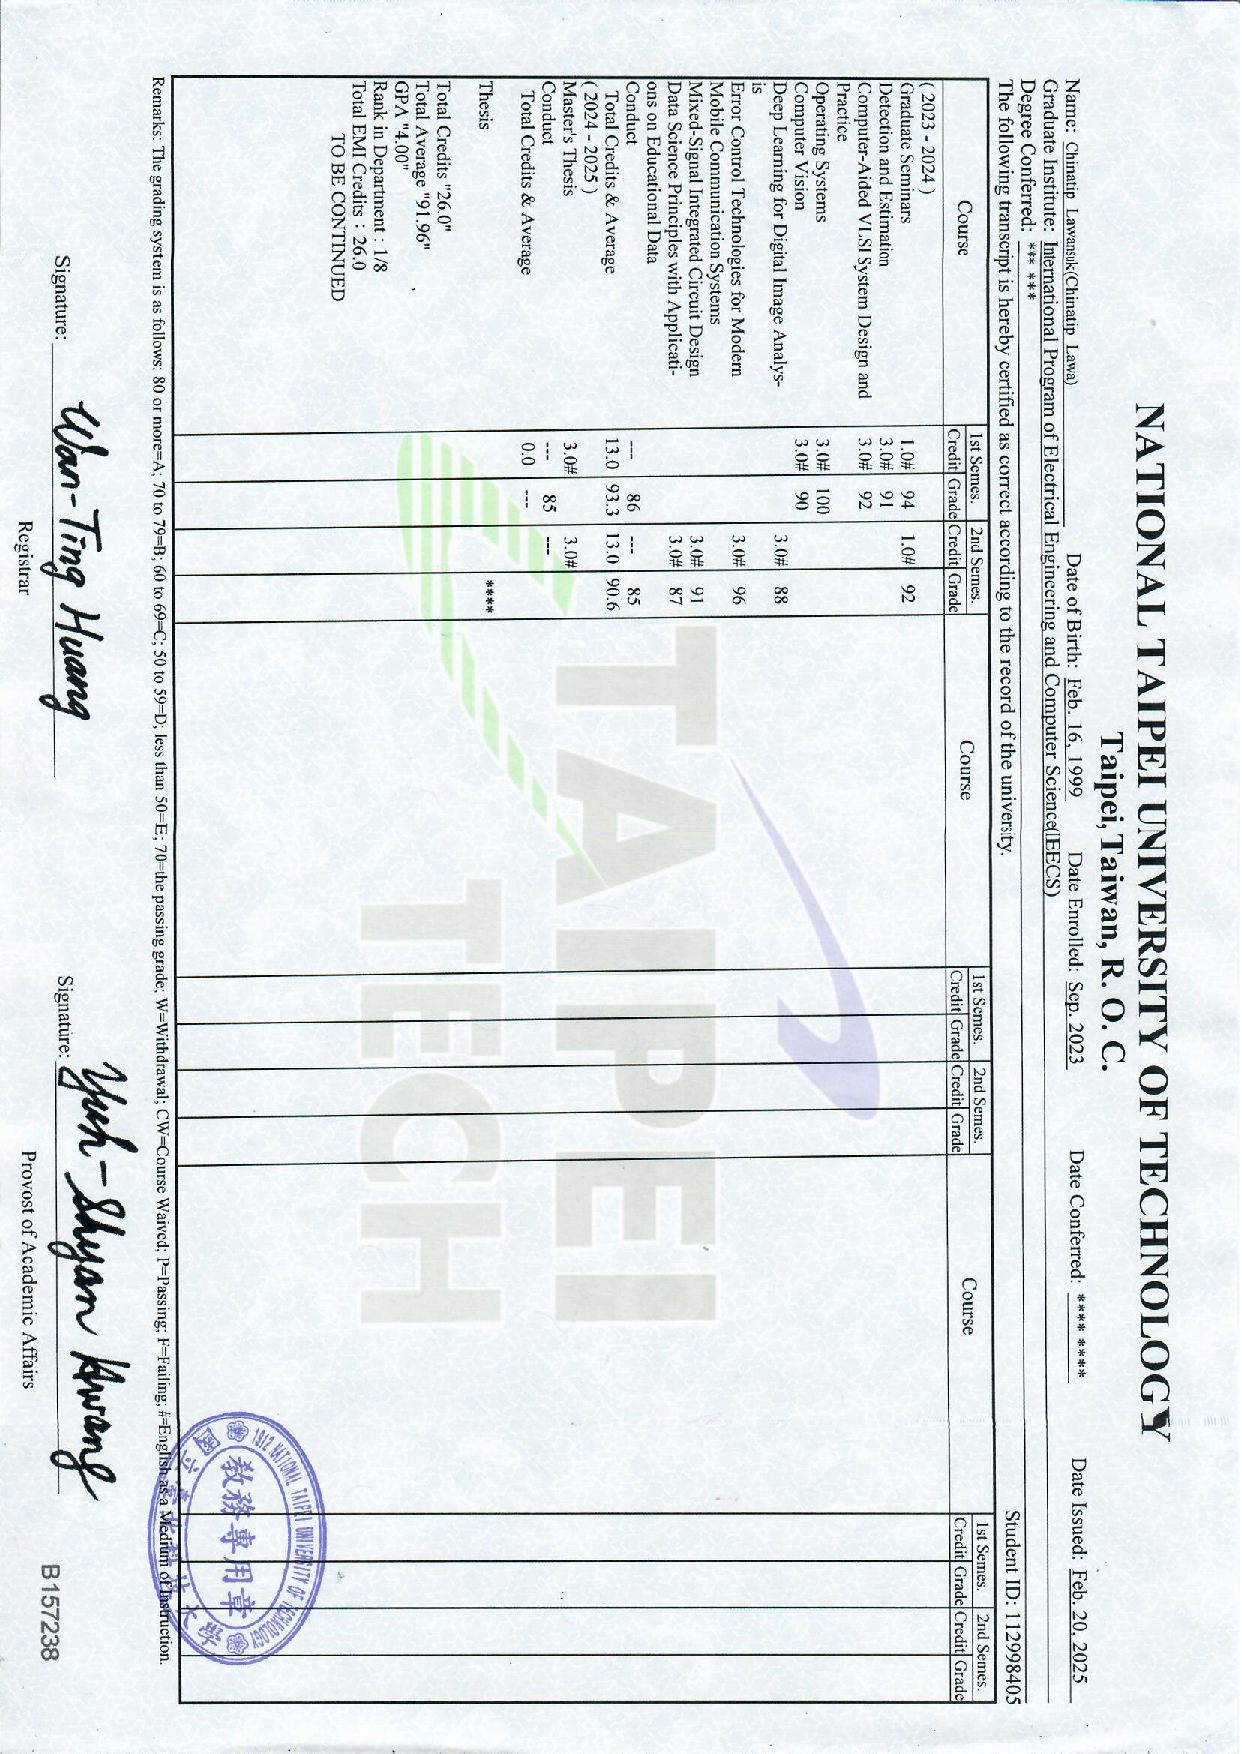
\includepdf[pages=-]{resources/Transcript_Chinatip_2025_rotated.pdf}
% 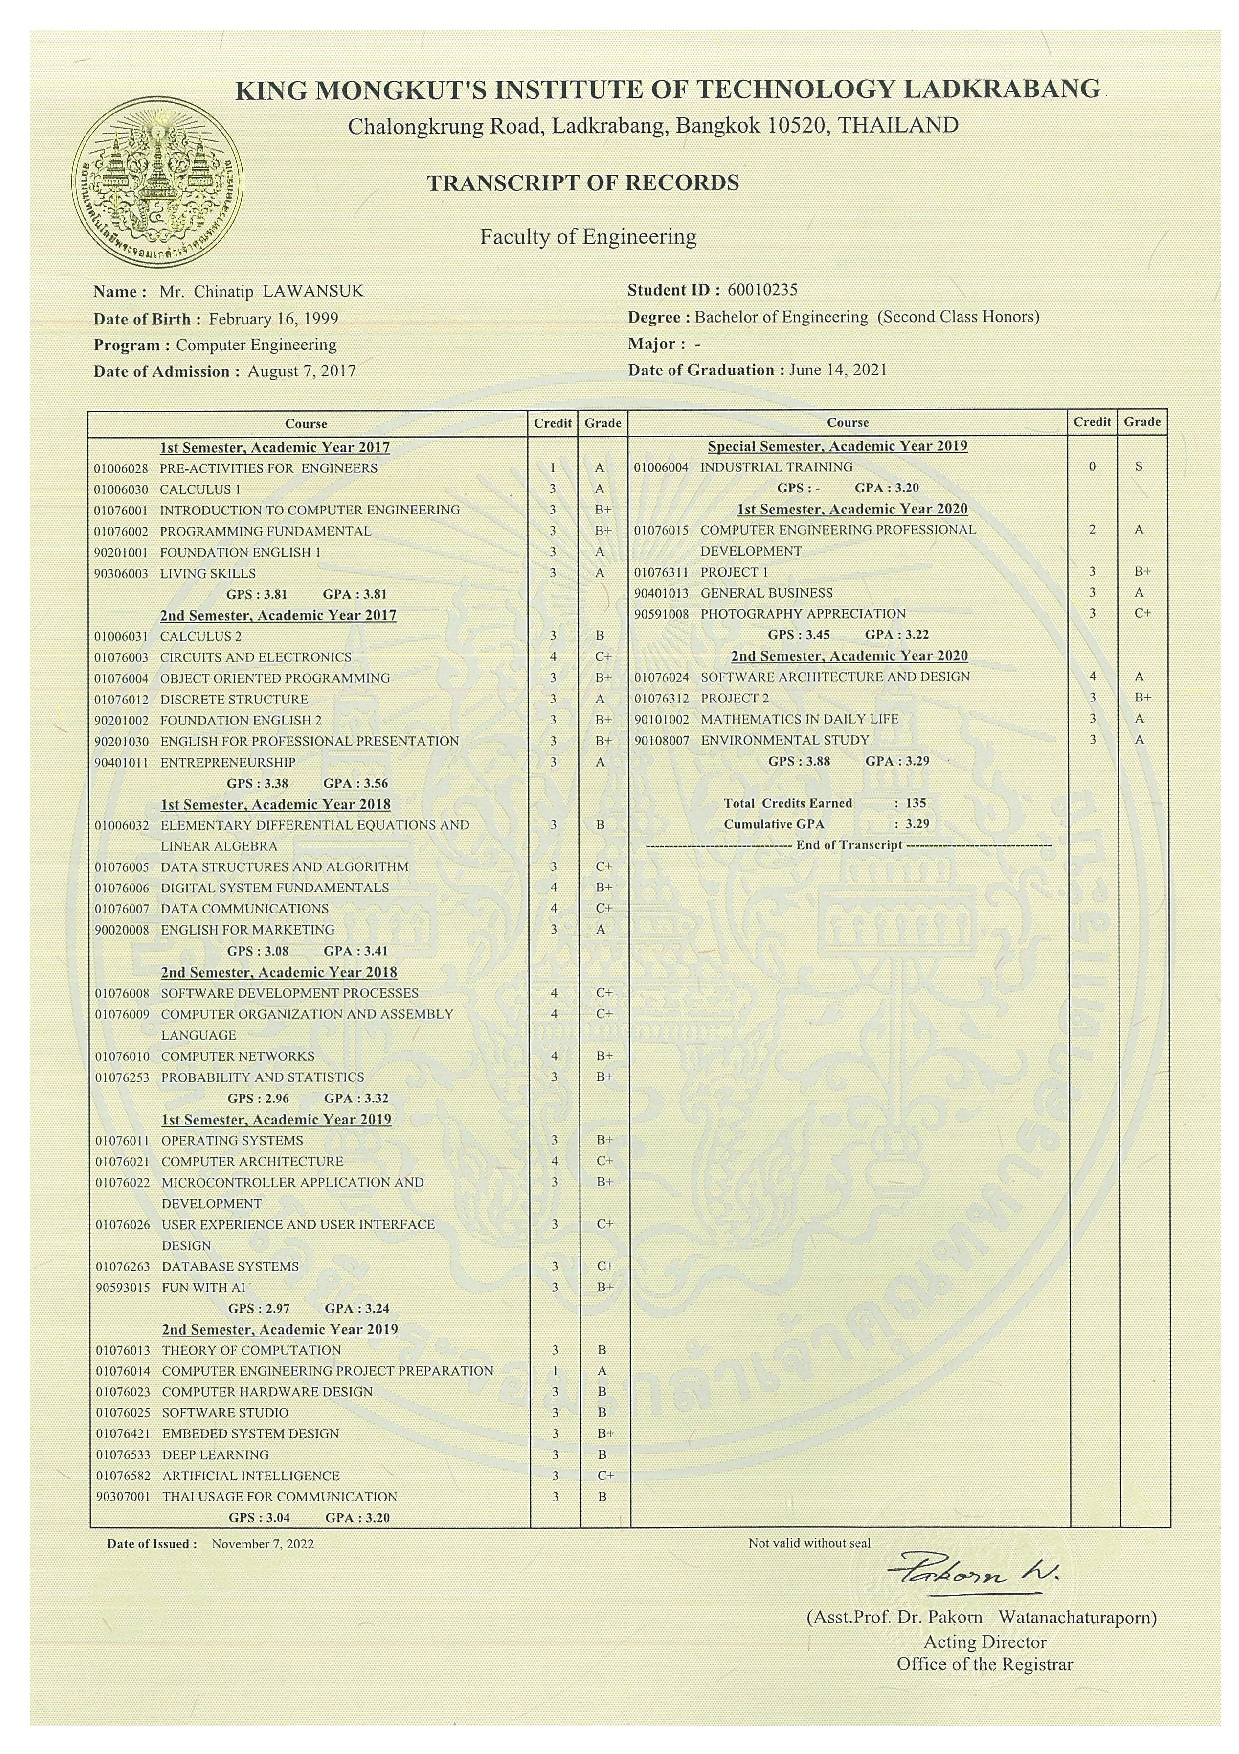
\includepdf[pages=-]{resources/Transcript_EN_KMITL.pdf}
% 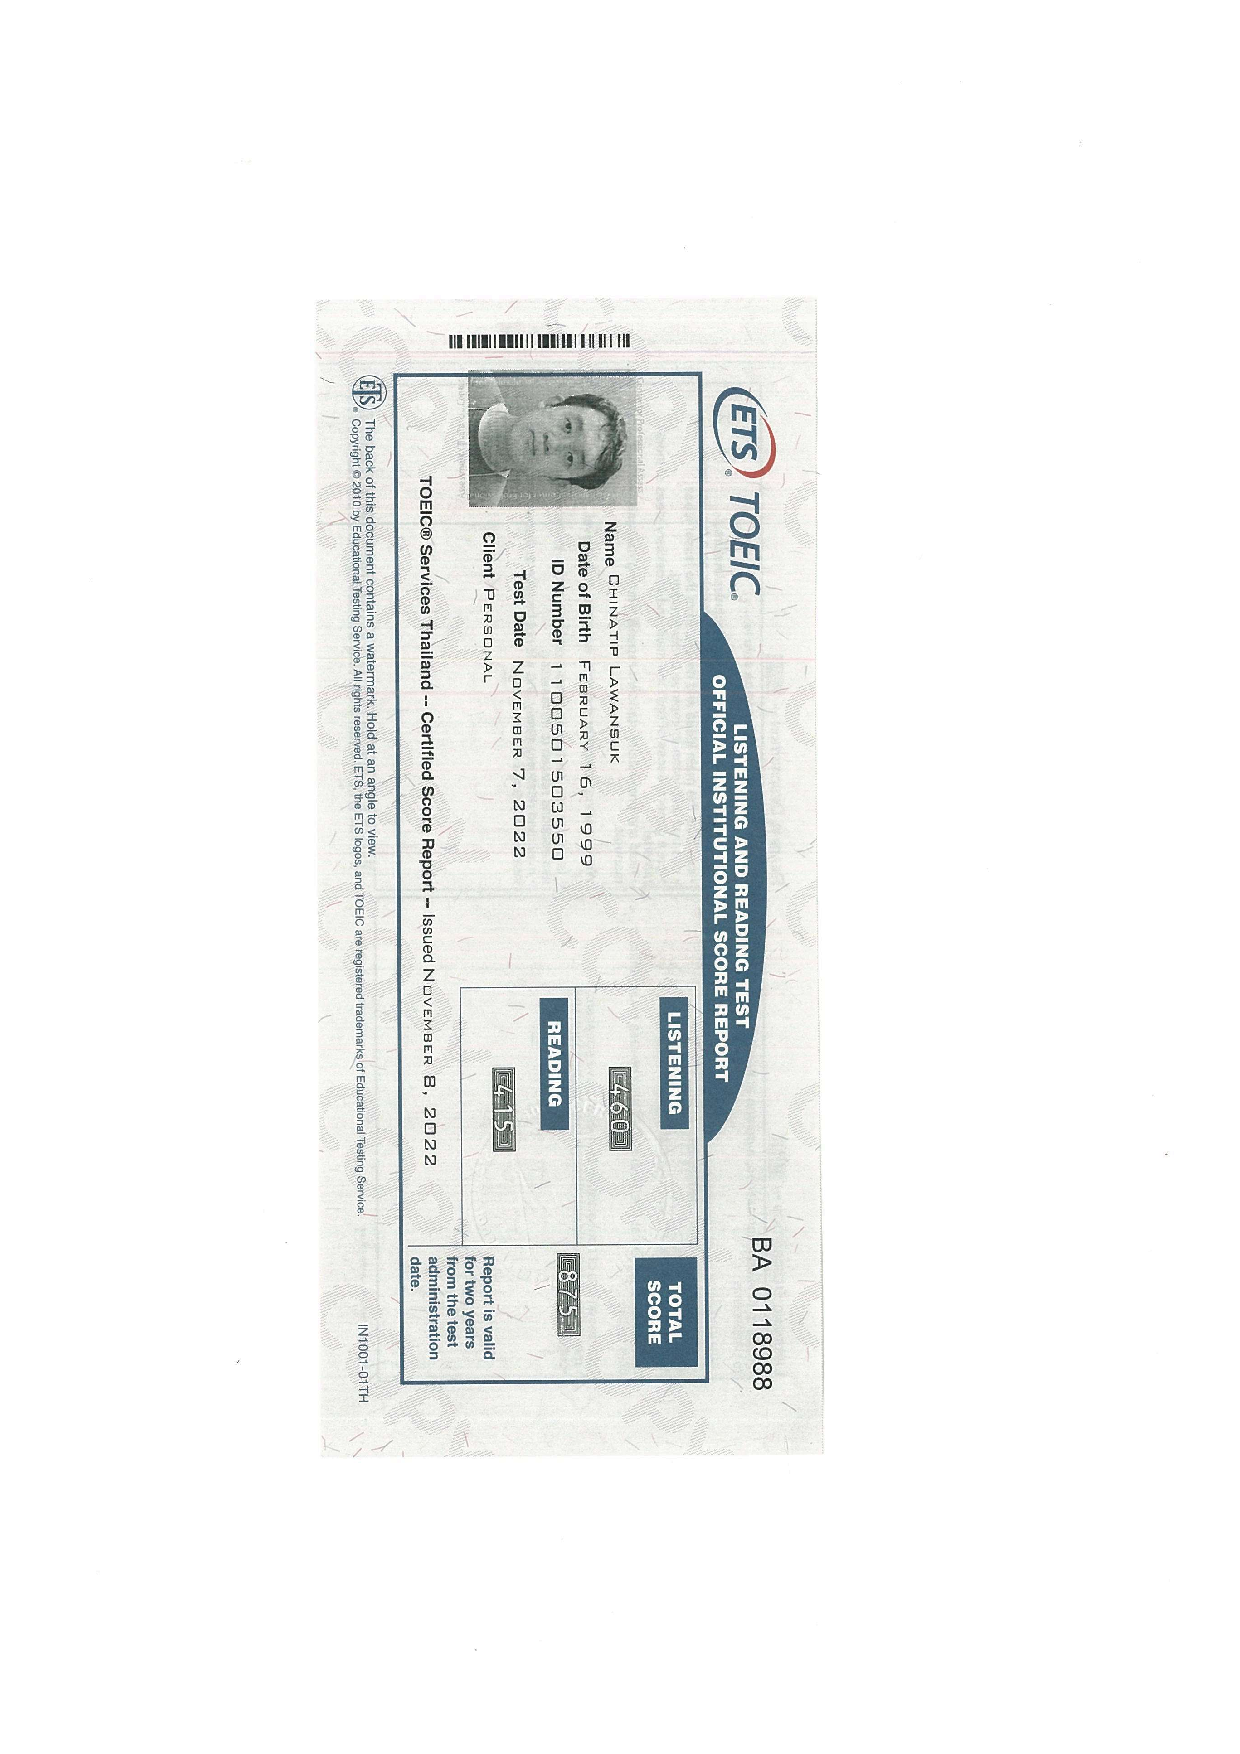
\includepdf[pages=-]{resources/TOEIC_Chinatip.pdf}







\end{document}